%-------------------------------------------------------------------------------
% TEMPLATE FOR UCL MSc THESIS
% (c) Paul Oswald, 2023

% This is a template for a MSc Thesis document, based on a Microsoft Word template given 
% by the Department of Medical Physics and Biomedical Engineering, UCL. 
%------------------------------------------------------------------------------- 


% ------------------ DOCUMENT SETUP ------------------ 
% The document class defines the document type (report) and sets the font size (12pt)
\documentclass[12pt]{report}
\author{Hanting Liu}


% Inputs the Document Packages
\input{_Packages}

% keep figure reference number consistent
\usepackage{notoccite}
\usepackage{amssymb}


% Hyperlink
\usepackage{hyperref}

% table 1
\usepackage{adjustbox}

% table 2
\usepackage{tabularx}
\usepackage{array}

% table 4
\usepackage{multirow}
\usepackage[normalem]{ulem}
\usepackage{booktabs}
\usepackage[mathscr]{eucal}
\usepackage{graphicx}
\usepackage[normalem]{ulem}
\useunder{\uline}{\ul}{}

% Controls how many subsections the document can take
%  and how many of those will get put into the contents pages.
\setcounter{secnumdepth}{3}
\setcounter{tocdepth}{3}

% Line Spacing
\setstretch{1.5}

% Psudo code
\usepackage{algorithm}
\usepackage{algorithmic}


% Places a dot after Chapter/Section/Subsection number in Table of Contents
\renewcommand{\cftchapaftersnum}{.}
\renewcommand{\cftsecaftersnum}{.}
\renewcommand{\cftsubsecaftersnum}{.}

%  Customize Dot spacing in Table of Contents/List of Figures/Tables
\renewcommand{\cftdotsep}{0.3}


% Line Break Properties
\tolerance=1
\emergencystretch=\maxdimen
\hyphenpenalty=10000
\hbadness=10000


% Formatting Table of Contents/Lists titles
\renewcommand{\contentsname}{\bfseries\LARGE{CONTENTS}}
\renewcommand{\listfigurename}{\bfseries\LARGE{LIST OF FIGURES}}
\renewcommand{\listtablename}{\bfseries\LARGE{LIST OF TABLES}}

% Signature Line for the declaration
\newbox\namebox
\newdimen\signboxdim

\def\signature#1{%
    \setbox\namebox=\hbox{#1}
    \signboxdim=\dimexpr(\wd\namebox+3cm)
    \parbox[t]{\signboxdim}{%
        \centering
            \hrulefill\\    % for a line
            #1
        \par}%
    }

% Title Formatting customization
\titleformat{\chapter}{\normalfont\bfseries\LARGE}{\thechapter.}{1em}{\MakeUppercase}

\titleformat{\section}{\normalfont\bfseries\large}{\thesection.}{1em}{\MakeUppercase}
\titlespacing*{\section} {0pt} {0pt} {15pt} % left, before, after

\titleformat{\subsection}{\normalfont\bfseries\large}{\thesubsection.}{1em}{}
\titlespacing*{\subsection} {0pt} {10pt} {10pt}

\titleformat{\subsubsection}{\normalfont\bfseries\large}{\thesubsubsection.}{1em}{}
\titlespacing*{\subsubsection} {0pt} {10pt} {10pt}


% HEADER AND FOOTER
\pagestyle{fancy}  % Set Page Style (Header and Footer Style)
\fancyhf{}  % Clears the header and footer (from the default info)

% Header
\renewcommand{\headrulewidth}{0pt}  % Removes the default Horizontal Line in Header
% Optional Headers
%\fancyhead[L]{}
%\fancyhead[R]{2022/2023}

% Footer
\fancyfoot[C]{\thepage} % Page Number

% Change figure numbering per section
\numberwithin{figure}{chapter}

%Acronym entries
% \makeglossaries
% \newacronym{US}{US}{Ultrasound}


%  -------------------------------------------------
%  --------- The document starts from here --------- 
%  -------------------------------------------------
\begin{document}


% ------------------  TITLE PAGE -------------------
\begin{titlepage}
\begin{center}
    % UCL IMAGE
    \vspace*{-1cm}
    \noindent
    \makebox[\textwidth][l]{%
      
\includegraphics[width=0.2\paperwidth]{Images/uom_logo.pdf}%
    }
    
    \vspace{2.3cm}
    
    % Title
    {\relscale{1.19}{A thesis submitted in partial fulfilment of the requirements for the degree of Master of Science (MSc) in}}

    \vspace{1cm}
    {\relscale{1.15}\textbf{HEALTH DATA SCIENCE\\}}
    \vspace{0.3cm}
    {\relscale{1.15}\textbf{UNIVERSITY OF MANCHESTER\\}}
    \vspace{2.4cm}
    
    {\relscale{1.19}{Are Stronger Multimodal Large Language Models Better at Recognising Their Failures?\\[0.3cm] A Zero-Shot Evaluation Across Histopathology, Radiology, and Prostate Assessment}}\\
    %\vspace{0.1cm}
    By\\
    %\vspace{0.1cm}
    Hanting LIU\\
    \vspace{0.9cm}
    {\begin{singlespace}Supervisor: Mobarak Hoque\\
    \end{singlespace}}
\end{center}
{\raggedleft\vfill{\begin{singlespace}
     Faculty of Biology, Medicine\\
  and Health\\
\end{singlespace}
 UNIVERSITY OF MANCHESTER\\
 \begin{singlespace}
 Date of submission: August 2026\\
 Word count: TBC\\
 \end{singlespace}
}\par
}
\end{titlepage}

% ----------------------  DECLARATION -----------------------
\newpage
\chapter*{Declaration} % the Asterix (*) indicates that this section will be added to the table of contents but no number will be present beside it.
\addcontentsline{toc}{chapter}{Declaration}
I, Hanting Liu confirm that the work presented in this report is my own. Where information has been derived from other sources, I confirm that this has been indicated in the report.
\vspace*{3cm}

\noindent\signature{Hanting Liu}
\newpage
% ----------------------  ABSTRACT -----------------------
\newpage
\chapter*{Abstract} 
\addcontentsline{toc}{chapter}{Abstract}
\input{Abstract}

% -------------------  IMPACT STATEMENT --------------------
\newpage
\chapter*{Impact Statement}
\addcontentsline{toc}{chapter}{Impact Statement}
This dissertation evaluates whether healthcare vision-language models can identify answers that are likely to be unreliable under a reproducible benchmark protocol. The work may inform safer evaluation of systems intended for diagnostic support, pathology review, radiology questioning, or treatment-related decision support by showing why answer quality and failure awareness should be reported separately. It does not validate a clinical device, establish patient benefit, or show that any model is clinically safe. The failure endpoint is based on reference-matching metrics rather than expert adjudication, and the selective results are not clinical referral thresholds. Any future healthcare use would require expert-labelled errors, calibration, subgroup analysis, patient-level validation, prospective workflow testing, and assessment of missed harmful cases.



% -----------------  ACKNOWLEDGEMENTS  -------------------
\newpage
\chapter*{Acknowledgements}
\addcontentsline{toc}{chapter}{Acknowledgements}
I would like to thank my supervisor and the teaching staff of the MSc Health Data Science programme for their guidance during this project. I also thank the open-source communities and dataset creators whose models, benchmarks, and documentation made the experiments possible. Any remaining errors in the analysis or interpretation are my own.



% ------------------  TABLE OF CONTENTS --------------------
\newpage
\tableofcontents 


% -------------------  LIST OF FIGURES --------------------
\newpage  
\listoffigures%}
\addcontentsline{toc}{chapter}{List of Figures}


% -------------------  LIST OF TABLES ---------------------
\newpage
\listoftables%}
\addcontentsline{toc}{chapter}{List of Tables}


% -------------------  INTRODUCTION / LITERATURE REVIEW  ---------------------
\chapter{Introduction and Literature Review}
\input{Introduction}
\input{Background}

% -------------------  CASE / HYPOTHESIS / AIMS / OBJECTIVES  ---------------------
\chapter{Research Question and Objectives}
This chapter converts the gap identified in the literature into a focused research plan. It defines the clinical case, research question, hypotheses, objectives, and the limits of the evidence required to answer the question.

\section{Clinical Case for the Study}

Healthcare VLMs may support diagnosis, pathology review, clinical communication, and treatment planning, but a useful human-in-the-loop system must do more than generate fluent answers. It should also provide a signal when an answer should be withheld or referred for expert review. This matters at case level: a high average score can coexist with a small group of confident failures, and those cases may be more important to a clinician than a modest difference between benchmark means. Selective prediction formalises the separation between answering and abstaining \citep{geifman2017selective}, while responsible healthcare AI guidance stresses that errors and their consequences must be evaluated directly \citep{wiens2019donoharm}. Medical image questions make the distinction concrete: sampled answers may be mutually consistent but still be wrong or unrelated to the question, so consistency cannot substitute for validity \citep{carlini2026qasnne}. The intended use of a detector is therefore not to replace clinical judgement, but to provide evidence for deciding which cases require it. This dissertation asks that preclinical evaluation question and does not claim deployment readiness, patient benefit, or clinical safety.

\section{Problem Statement}

Reference metrics describe how closely a greedy answer matches a reference, but they do not show whether the model can identify its own weak outputs. Failure detection uses a different source of evidence: a score derived from sampled answers must rank metric-defined failures above non-failures. The detector score and the failure label must remain separate; otherwise the evaluation would reward a method for reproducing a target that it helped define. Semantic uncertainty can improve over exact string agreement, yet it remains sensitive to the model, task, and data distribution \citep{farquhar2024semanticentropy,ovadia2019uncertainty}. The unresolved problem is whether models that rank highly for answer generation also rank highly for failure detection when the checkpoints, prompts, decoding rules, references, and failure definition are held constant. Without this control, an apparent model difference could come from the evaluation rather than the model. PathVQA, VQA-RAD, and ProstateMM-CHIMERA provide equal but different pathology, radiology, and prostate assessment settings in which to examine that relationship \citep{he2020pathvqa,lau2018vqarad,chimera2025task1}.

\section{Research Question}

The primary research question is: \emph{Are healthcare VLMs with stronger answer-generation performance also better at recognising their unreliable answers in zero-shot medical visual question answering?} For model $m$ and dataset $d$, answer performance is represented by $\mathbf{A}_{m,d}=(\mathrm{BLEU1},\mathrm{BLEU2},\mathrm{ROUGE\mbox{-}L},\mathrm{METEOR})$, while detector $k$ is represented by $\mathbf{R}_{m,d,k}=(\mathrm{AUROC},\mathrm{AUPRC},\mathrm{selective\ performance})$. The analysis asks whether the model ordering produced by $\mathbf{A}$ agrees with that produced by $\mathbf{R}$. Agreement would mean that the strongest answer generator also produces the most informative failure signal in the same setting. Divergence would mean that answer performance cannot stand in for reliability evaluation, while a changing relationship would make the conclusion dataset-dependent. Four supporting questions follow: how the three models rank on answer quality; how well their sampled outputs detect operational failures; whether the two rankings agree within each dataset; and whether the relationship changes across the three medical settings.

\section{Hypotheses}

The main working hypothesis is that answer-generation strength and failure awareness are related but distinct, so their model rankings will not show uniform agreement across all datasets. A second hypothesis is that detector performance depends on the model and dataset because architectures, training, image modalities, question forms, and clinical context differ; uncertainty is known to change under distribution shift \citep{ovadia2019uncertainty}. A third expectation is that an informative detector will improve retained answer quality and reduce the operational failure rate when high-scoring cases are rejected compared with random selection. The first hypothesis is supported by at least one clear ranking divergence, the second by changes in model or detector order across datasets, and the third by improvement over random ranking at matched coverage. Uniform ranking agreement would weaken the first hypothesis, while selective performance close to random would weaken the third. These are descriptive hypotheses about ranking and selective behaviour, not confirmatory tests of patient outcomes.

\section{Aim and Objectives}

The aim is to determine whether stronger zero-shot answer generation can be treated as evidence of stronger operational failure awareness in healthcare VLMs. Six linked objectives answer this aim: (1) evaluate Qwen2.5-VL-3B-Instruct, LLaVA-1.5-7B, and MedGemma-4B-it under a controlled zero-shot protocol; (2) measure greedy answers with BLEU-1, BLEU-2, ROUGE-L, and METEOR; (3) apply one reproducible operational failure rule to all outputs; (4) derive AFD frequency, Semantic AFD, and question-aligned uncertainty from three sampled answers, with a random baseline; (5) evaluate discrimination using AUROC and AUPRC and examine selective performance at fixed coverages; and (6) compare answer-quality and failure-detection rankings within each dataset and across settings. Together, these steps form one evidence chain from controlled generation to answer measurement, failure definition, detector evaluation, and final ranking comparison.

\section{Scope and Definitions}

The study is retrospective, quantitative, comparative, and preclinical. It uses 6,719 PathVQA test items, 451 VQA-RAD test items, and 42 ProstateMM-CHIMERA task records from 14 patients. Each dataset has a domain-specific prompt that is fixed across the three models, and no checkpoint is fine-tuned on the test split. One greedy output is evaluated, while three sampled outputs are used only for detector scores. \emph{Answer quality} means reference agreement under the four stated metrics. An \emph{operational failure} occurs when item-level ROUGE-L is below 20\% and METEOR is below 10\%. \emph{Failure awareness} means that a detector ranks these failures above non-failures; uncertainty is the predictor, not the label. Scores are calculated on their standard normalised scales and displayed as percentages, with differences reported in percentage points.

\section{Expected Contribution}

The contribution is an evaluation framework rather than a new VLM or uncertainty algorithm. It places answer generation and operational failure detection in one controlled comparison without merging them into a single score, compares three differently trained VLMs across three equal medical settings, and links detector discrimination to selective performance. Agreement between the two rankings would suggest that answer strength provides some evidence about failure awareness under the tested conditions; divergence would show that the properties require separate evaluation; and a changing relationship would show that conclusions depend on task and data distribution. Because the failure label is a lexical proxy rather than expert-adjudicated harm, the findings describe metric-defined reliability and cannot establish grounding, calibration for deployment, patient safety, or improved clinical decisions.


% -------------------  DESIGN OF STUDY OR METHOD  ---------------------
\chapter{Methods}
\input{Methodology}
This section describes the three datasets used by the common evaluation framework. They are analysed separately so that the much larger PathVQA split does not dominate the other settings.

\section{Dataset Selection}

PathVQA provides a large histopathology benchmark, VQA-RAD changes the image domain to radiology, and ProstateMM-CHIMERA adds patient-linked clinical context to a prostate assessment task. Differences in image type, question form, answer length, and context allow the stability of model and detector rankings to be examined without treating any dataset as more important than another. The comparison tests dataset dependence; it does not prove clinical generalisation.

\begin{table}[htbp]
    \centering
    \caption{Dataset setting, unit of analysis, and evaluation size.}
    \label{tab:dataset-overview}
    \small
    \begin{tabularx}{\textwidth}{lXXr}
        \toprule
        Dataset & Image setting & Unit of analysis & Test records \\
        \midrule
        PathVQA & Histopathology & Image-question pair & 6,719 \\
        VQA-RAD & Radiology & Image-question pair & 451 \\
        ProstateMM-CHIMERA & Prostate assessment & Patient-linked task record & 42 \\
        \bottomrule
    \end{tabularx}
\end{table}

\section{PathVQA}

PathVQA contains pathology images with questions about organs, tissues, appearances, and disease-related concepts \citep{he2020pathvqa}. The experiment uses the complete official test split of 6,719 image-question pairs; no item is used for adaptation or model selection. Each record provides an image, question, and reference answer, and the same ordered records are evaluated by all three models. Figure~\ref{fig:pathvqa-example} illustrates the short, locally focused answer style and the potential difficulty of lexical evaluation when valid medical terms have different surface forms.

\begin{figure}[htbp]
    \centering
    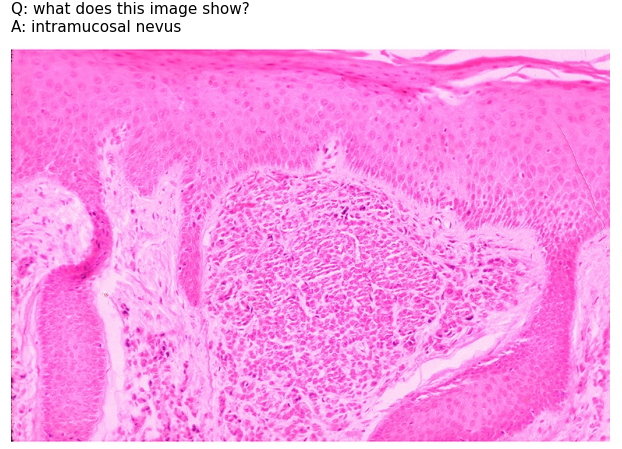
\includegraphics[width=0.82\textwidth]{Images/dataset_example_pathvqa.png}
    \caption[Representative PathVQA record]{Representative PathVQA record. Source: PathVQA \citep{he2020pathvqa}.}
    \label{fig:pathvqa-example}
\end{figure}

\section{VQA-RAD}

VQA-RAD contains radiology images with clinician-generated closed and open questions \citep{lau2018vqarad}. Its official test split contains 451 image-question pairs, all evaluated zero-shot with one greedy and three sampled answers. The modality, terminology, and answer distribution differ from PathVQA, making it a distinct test of the relationship between answer quality and failure detection. The smaller sample requires caution when interpreting close differences, and the dataset does not reproduce a complete radiology reporting workflow.
The final per-record exports were checked separately for this split. Each model file contains the same 451 indices (0--450), no empty greedy answers, and three sampled answers per item. The files use the model keys \texttt{qwen2\_5\_vl\_3b}, \texttt{llava\_1\_5\_7b}, and \texttt{medgemma\_4b\_it}; these keys are used to identify the final checkpoints in the analysis.

\begin{figure}[htbp]
    \centering
    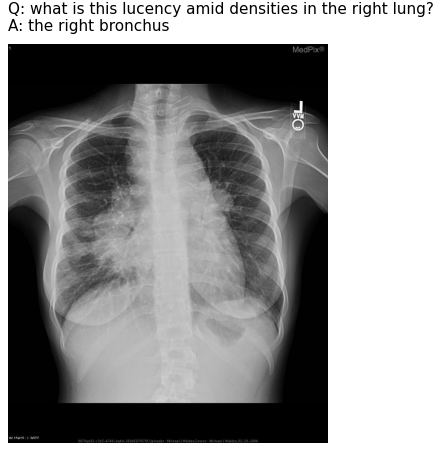
\includegraphics[width=0.74\textwidth]{Images/dataset_example_vqarad.png}
    \caption[Representative VQA-RAD record]{Representative VQA-RAD record. Source: VQA-RAD \citep{lau2018vqarad}.}
    \label{fig:vqarad-example}
\end{figure}

\section{ProstateMM-CHIMERA}

ProstateMM-CHIMERA is the project evaluation package derived from CHIMERA 2025 Task 1 on prostate cancer biochemical recurrence prediction \citep{chimera2025task1}; it is not presented as a separately published dataset under that exact name. Records combine histopathology, a focused question, and structured clinical context. The full package contains 285 task records from 95 patients, divided into 201 training, 42 validation, and 42 test records, with three records per patient. Only the held-out test records from 14 patients are used, so results are task-record estimates rather than independent patient-level estimates. Figure~\ref{fig:chimera-example} shows the more decision-oriented answer style.

\begin{figure}[htbp]
    \centering
    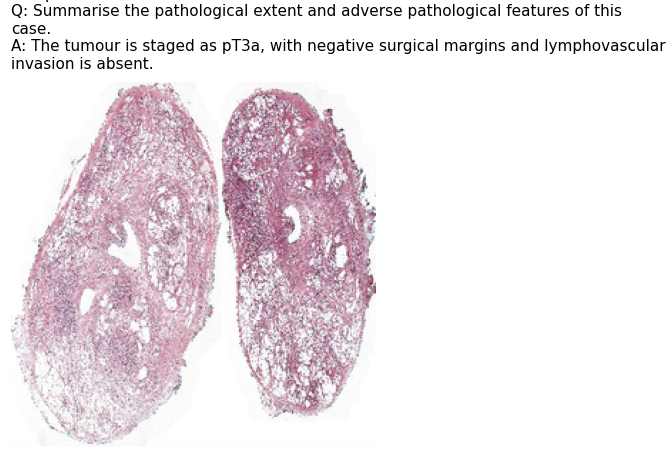
\includegraphics[width=0.82\textwidth]{Images/dataset_example_chimera.png}
    \caption[Representative ProstateMM-CHIMERA record]{Representative record from the project package derived from CHIMERA 2025 Task 1 \citep{chimera2025task1}.}
    \label{fig:chimera-example}
\end{figure}

\section{Prompts and Processing}

Each dataset uses one domain-specific prompt fixed across Qwen2.5-VL-3B-Instruct, LLaVA-1.5-7B, and MedGemma-4B-it. The prompts define the available evidence and request concise answers; ProstateMM-CHIMERA adds clinical context but excludes target facts and references from the model input.

\subsection{PathVQA Prompt}

\begin{quote}
You are a professional pathologist specialized in histopathology. You are answering visual questions based on pathology slide images. Use the given image, the question, and appropriate pathology knowledge to answer. For yes/no questions, answer only `yes' or `no'. For other questions, answer with the shortest medically appropriate phrase or term. Do not repeat the question. Do not provide explanations or unrelated information.
\end{quote}

\subsection{VQA-RAD Prompt}

\begin{quote}
You are a medical imaging specialist experienced in radiology. You are answering visual questions based on radiological images. Use the image, the question, and appropriate radiological knowledge to answer. For yes/no questions, answer only `yes' or `no'. For other questions, provide a concise radiological answer using a short phrase. Do not repeat the question. Do not add uncertain diagnosis, treatment advice, or unrelated details.
\end{quote}

\subsection{ProstateMM-CHIMERA Prompt}

\begin{quote}
You are a specialist pathologist experienced in prostate cancer assessment. You are answering visual questions based on prostate histopathology images and the provided clinical context. Use only the image, the question, and the clinical context to answer. For biochemical recurrence prediction or other yes/no questions, answer only `yes' or `no'. For grading, extent assessment, or other open-ended questions, answer with the most concise clinically appropriate phrase or value. Do not repeat the question. Do not provide long explanations, reasoning steps, or unrelated information.
\end{quote}

Generated text is cleaned by removing common assistant prefixes, normalising whitespace, and retaining the first non-empty line; case and punctuation are normalised only for scoring, and predictions are not rewritten to match references.

\section{Records and Data Quality}

The unit of analysis is an image-question pair for PathVQA and VQA-RAD and a patient-linked task record for ProstateMM-CHIMERA. All three models evaluate the same source records, producing 20,157 PathVQA, 1,353 VQA-RAD, and 126 ProstateMM-CHIMERA greedy model-item outputs, each paired with three samples. Source indices preserve joins between answers, labels, and detector scores. Image paths, required fields, splits, cache size, and duplicate records are checked before scoring; final PathVQA results use records marked \texttt{test\_full}, while ProstateMM-CHIMERA uses \texttt{test}. The complete VQA-RAD per-record exports permit direct calculation of failure prevalence, while coverage rows remain selective operating points rather than prevalence estimates. The small prostate test and within-patient dependence remain explicit limits.


% -------------------  RESULTS  ---------------------
\chapter{Results}
This chapter reports answer quality, operational failure detection, and their relationship across the three datasets. All bounded values are displayed as percentages and differences as percentage points; calculations remain on standard normalised scales. Results are descriptive because one inference run is available and no confidence intervals or significance tests were calculated.

\section{Overall Experimental Results}

Table~\ref{tab:overall-result-pattern} summarises the central result. PathVQA gives a metric-dependent answer ranking: Qwen2.5-VL-3B-Instruct leads BLEU-1 and BLEU-2, while MedGemma-4B-it leads ROUGE-L and METEOR; Qwen2.5-VL-3B-Instruct has the highest detector AUROC. VQA-RAD shows clearer divergence because MedGemma-4B-it leads three answer metrics but Qwen2.5-VL-3B-Instruct leads failure detection. ProstateMM-CHIMERA instead shows alignment, with MedGemma-4B-it leading three answer metrics and AUROC. The relationship is therefore not constant across metrics or datasets, and the small patient-linked prostate result requires particular caution.

\begin{table}[htbp]
    \centering
    \caption{Central comparison between answer quality and failure detection.}
    \label{tab:overall-result-pattern}
    \small
    \begin{tabularx}{\textwidth}{lXXrl}
        \toprule
        Dataset & Answer-quality leader & Best detector (model; method) & AUROC & Relationship \\
        \midrule
        PathVQA & Qwen2.5-VL-3B-Instruct on BLEU; MedGemma-4B-it on ROUGE-L/METEOR & Qwen2.5-VL-3B-Instruct; question-aligned & 81.20\% & Metric-dependent \\
        VQA-RAD & MedGemma-4B-it on three metrics & Qwen2.5-VL-3B-Instruct; Semantic AFD & 69.43\% & \textbf{Divergent} \\
        ProstateMM-CHIMERA & MedGemma-4B-it on three metrics & MedGemma-4B-it; question-aligned & 93.88\% & \textbf{Aligned} \\
        \bottomrule
    \end{tabularx}
\end{table}

\section{Answer Quality on PathVQA}

Table~\ref{tab:answer-quality-all} shows all answer results. On PathVQA, Qwen2.5-VL-3B-Instruct leads BLEU-1 at 25.29\% and BLEU-2 at 1.38\%, whereas MedGemma-4B-it leads ROUGE-L at 34.77\% and METEOR at 17.73\%; LLaVA-1.5-7B is lowest on all four metrics. Relative to Qwen2.5-VL-3B-Instruct, MedGemma-4B-it is 3.03 percentage points higher on ROUGE-L and 1.63 points higher on METEOR but 5.78 points lower on BLEU-1 and 0.95 points lower on BLEU-2. Answer strength on this dataset therefore depends on the metric, so all four measures are retained rather than combined into one accuracy value.

\begin{table}[htbp]
    \centering
    \caption{Answer-quality comparison. Bold and underlined values are best and second-best within each dataset and metric.}
    \label{tab:answer-quality-all}
    \begin{tabularx}{\textwidth}{lXrrrr}
        \toprule
        Dataset & Model & BLEU-1 & BLEU-2 & ROUGE-L & METEOR \\
        \midrule
        \multirow{3}{*}{PathVQA}
        & Qwen2.5-VL-3B-Instruct & \textbf{25.29\%} & \textbf{1.38\%} & \underline{31.74\%} & \underline{16.10\%} \\
        & LLaVA-1.5-7B & \underline{19.89\%} & \underline{0.74\%} & 26.75\% & 13.53\% \\
        & MedGemma-4B-it & 19.51\% & 0.43\% & \textbf{34.77\%} & \textbf{17.73\%} \\
        \midrule
        \multirow{3}{*}{VQA-RAD}
        & Qwen2.5-VL-3B-Instruct & \underline{39.37\%} & \textbf{8.49\%} & \underline{48.16\%} & \underline{25.94\%} \\
        & LLaVA-1.5-7B & 38.41\% & 4.88\% & 40.25\% & 20.42\% \\
        & MedGemma-4B-it & \textbf{40.18\%} & \underline{6.60\%} & \textbf{58.66\%} & \textbf{31.05\%} \\
        \midrule
        \multirow{3}{*}{ProstateMM-CHIMERA}
        & Qwen2.5-VL-3B-Instruct & \underline{25.54\%} & \underline{8.77\%} & \underline{19.56\%} & \textbf{22.48\%} \\
        & LLaVA-1.5-7B & 19.00\% & 2.18\% & 15.27\% & 13.90\% \\
        & MedGemma-4B-it & \textbf{62.24\%} & \textbf{28.57\%} & \textbf{21.86\%} & \underline{16.77\%} \\
        \bottomrule
    \end{tabularx}
\end{table}

\section{Answer Quality on VQA-RAD}

On VQA-RAD, MedGemma-4B-it leads BLEU-1, ROUGE-L, and METEOR, while Qwen2.5-VL-3B-Instruct leads BLEU-2 and LLaVA-1.5-7B is lowest throughout. MedGemma-4B-it's ROUGE-L of 58.66\% is 10.50 percentage points above Qwen2.5-VL-3B-Instruct and 18.41 points above LLaVA-1.5-7B. Its METEOR of 31.05\% is also highest. These within-dataset rankings support MedGemma-4B-it as the strongest answer generator on three measures, but higher absolute values than PathVQA do not prove that radiology is easier because answer style and reference distributions differ.

\section{Operational Failure Distribution}

The final per-record exports allow the operational failure prevalence to be reported for the complete test splits. These values are the proportion of records whose greedy answer falls below both fixed reference-matching thresholds; they are not clinical error rates. MedGemma-4B-it has the lowest prevalence on all three datasets, while Qwen2.5-VL-3B-Instruct has a lower prevalence than LLaVA-1.5-7B on VQA-RAD. This describes failure burden, not detector quality: a model can produce fewer metric-defined failures without ranking its remaining failures well. AUPRC is interpreted cautiously because it also depends on positive-class prevalence.

\begin{table}[htbp]
    \centering
    \caption{Operational failure prevalence in the complete test split. Values are percentages of all evaluated records and are not clinical error rates.}
    \label{tab:failure-prevalence}
    \begin{tabularx}{\textwidth}{lXrr}
        \toprule
        Dataset & Model & Test records & Failure prevalence \\
        \midrule
        PathVQA & Qwen2.5-VL-3B-Instruct & 6,719 & \underline{66.88\%} \\
        PathVQA & LLaVA-1.5-7B & 6,719 & 71.96\% \\
        PathVQA & MedGemma-4B-it & 6,719 & \textbf{62.94\%} \\
        VQA-RAD & Qwen2.5-VL-3B-Instruct & 451 & \underline{47.23\%} \\
        VQA-RAD & LLaVA-1.5-7B & 451 & 58.09\% \\
        VQA-RAD & MedGemma-4B-it & 451 & \textbf{36.81\%} \\
        ProstateMM-CHIMERA & Qwen2.5-VL-3B-Instruct & 42 & 54.76\% \\
        ProstateMM-CHIMERA & LLaVA-1.5-7B & 42 & \underline{42.86\%} \\
        ProstateMM-CHIMERA & MedGemma-4B-it & 42 & \textbf{33.33\%} \\
        \bottomrule
    \end{tabularx}
\end{table}

\section{Failure Detection Results}

On PathVQA, Qwen2.5-VL-3B-Instruct has the highest AUROC for every informed detector and reaches 81.20\% with question-aligned uncertainty (Table~\ref{tab:pathvqa-failure-detection}). AFD frequency is best by AUROC for LLaVA-1.5-7B at 69.55\% and MedGemma-4B-it at 68.63\%, whereas question-aligned uncertainty gives their highest AUPRC. Random AUROCs remain close to 50\%. At 50\% coverage, all selected best-AUROC conditions improve accepted ROUGE-L and reduce failure rate relative to random ranking (Table~\ref{tab:selective-gain-50}); the largest PathVQA change is Qwen2.5-VL-3B-Instruct, with ROUGE-L rising by 21.65 points and failure rate falling by 21.52 points.

\begin{table}[htbp]
    \centering
    \caption{Retained failure detectors on PathVQA. Bold and underlined values are best and second-best within each model.}
    \label{tab:pathvqa-failure-detection}
    \begin{tabularx}{\textwidth}{XXrr}
        \toprule Model & Detector & AUROC & AUPRC \\ \midrule
        Qwen2.5-VL-3B-Instruct & Question-aligned uncertainty & \textbf{81.20\%} & \textbf{90.71\%} \\
        Qwen2.5-VL-3B-Instruct & AFD frequency & \underline{79.38\%} & \underline{86.08\%} \\
        Qwen2.5-VL-3B-Instruct & Semantic AFD & 78.59\% & 85.61\% \\
        Qwen2.5-VL-3B-Instruct & Random baseline & 50.91\% & 66.78\% \\ \midrule
        LLaVA-1.5-7B & Question-aligned uncertainty & 64.76\% & \textbf{83.39\%} \\
        LLaVA-1.5-7B & AFD frequency & \textbf{69.55\%} & \underline{82.93\%} \\
        LLaVA-1.5-7B & Semantic AFD & \underline{66.06\%} & 80.97\% \\
        LLaVA-1.5-7B & Random baseline & 50.14\% & 71.78\% \\ \midrule
        MedGemma-4B-it & Question-aligned uncertainty & 62.96\% & \textbf{77.92\%} \\
        MedGemma-4B-it & AFD frequency & \textbf{68.63\%} & \underline{75.61\%} \\
        MedGemma-4B-it & Semantic AFD & \underline{64.17\%} & 72.73\% \\
        MedGemma-4B-it & Random baseline & 50.42\% & 62.87\% \\ \bottomrule
    \end{tabularx}
\end{table}

\begin{table}[htbp]
    \centering
    \caption{Gain over random ranking at 50\% coverage. Positive percentage-point values are favourable.}
    \label{tab:selective-gain-50}
    \small
    \begin{tabularx}{\textwidth}{lXXrr}
        \toprule Dataset & Model & Best detector & $\Delta$ROUGE-L & Failure-rate reduction \\ \midrule
        PathVQA & Qwen2.5-VL-3B-Instruct & Question-aligned & \textbf{21.65\%} & \textbf{21.52\%} \\
        PathVQA & LLaVA-1.5-7B & AFD frequency & 10.89\% & 10.32\% \\
        PathVQA & MedGemma-4B-it & AFD frequency & 12.79\% & 11.88\% \\ \midrule
        VQA-RAD & Qwen2.5-VL-3B-Instruct & Semantic AFD & \textbf{12.48\%} & \textbf{11.51\%} \\
        VQA-RAD & LLaVA-1.5-7B & Semantic AFD & 8.09\% & 7.07\% \\
        VQA-RAD & MedGemma-4B-it & Question-aligned & 3.11\% & 4.87\% \\ \midrule
        ProstateMM-CHIMERA & Qwen2.5-VL-3B-Instruct & Question-aligned & 6.13\% & 14.28\% \\
        ProstateMM-CHIMERA & LLaVA-1.5-7B & Question-aligned & 7.26\% & \textbf{28.57\%} \\
        ProstateMM-CHIMERA & MedGemma-4B-it & Question-aligned & \textbf{11.68\%} & \textbf{28.57\%} \\ \bottomrule
    \end{tabularx}
\end{table}

Figures~\ref{fig:performance-rejection-qwen}--\ref{fig:performance-rejection-medgemma} show that informed detectors usually improve PathVQA accepted ROUGE-L as exclusion increases. On ProstateMM-CHIMERA, question-aligned uncertainty improves all three models, whereas AFD frequency can perform below random for Qwen2.5-VL-3B-Instruct and LLaVA-1.5-7B, supporting dataset-specific detector selection.

\begin{figure}[htbp]
    \centering
    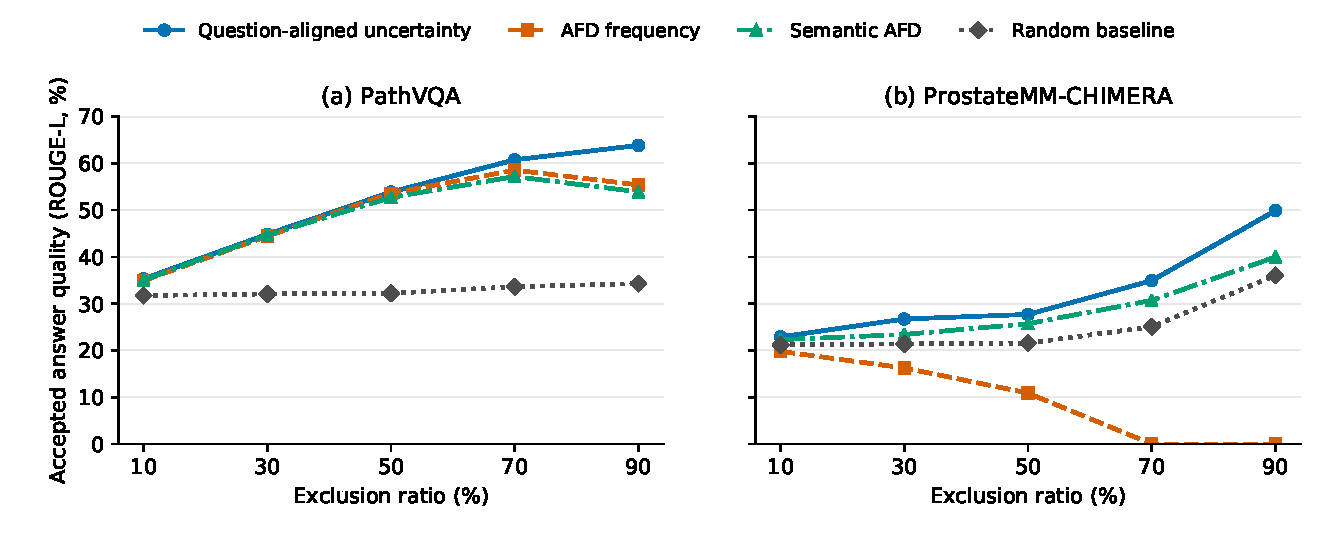
\includegraphics[width=0.92\textwidth]{Images/performance_rejection_qwen.pdf}
    \caption{Accepted ROUGE-L by exclusion for Qwen2.5-VL-3B-Instruct on PathVQA and ProstateMM-CHIMERA.}
    \label{fig:performance-rejection-qwen}
\end{figure}

\begin{figure}[htbp]
    \centering
    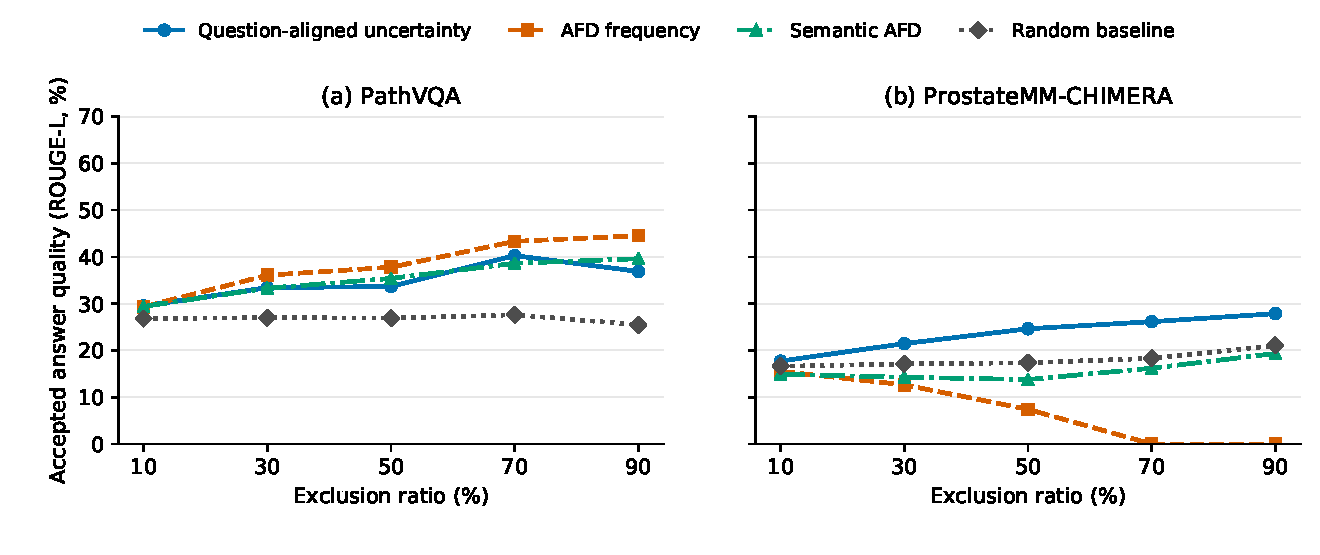
\includegraphics[width=0.92\textwidth]{Images/performance_rejection_llava.pdf}
    \caption{Accepted ROUGE-L by exclusion for LLaVA-1.5-7B on PathVQA and ProstateMM-CHIMERA.}
    \label{fig:performance-rejection-llava}
\end{figure}

\begin{figure}[htbp]
    \centering
    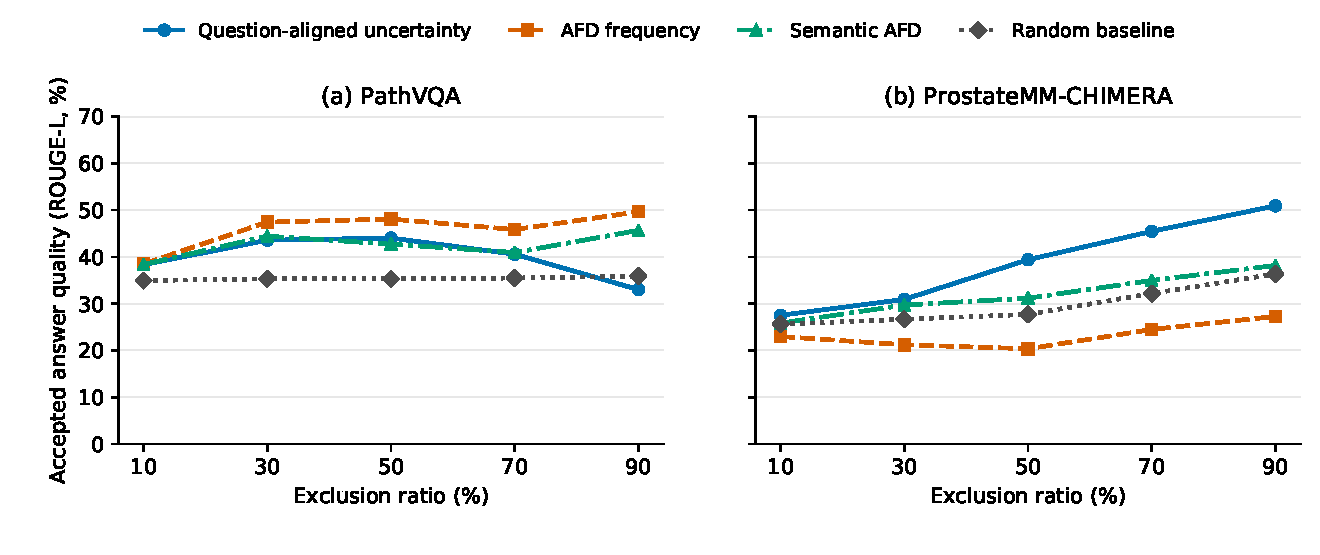
\includegraphics[width=0.92\textwidth]{Images/performance_rejection_medgemma.pdf}
    \caption{Accepted ROUGE-L by exclusion for MedGemma-4B-it on PathVQA and ProstateMM-CHIMERA.}
    \label{fig:performance-rejection-medgemma}
\end{figure}

\section{Model Ranking Across Dimensions}

Table~\ref{tab:best-detector-all} gives the best detector for every model and dataset. PathVQA ranks Qwen2.5-VL-3B-Instruct, LLaVA-1.5-7B, then MedGemma-4B-it by AUROC, agreeing with BLEU but conflicting with ROUGE-L and METEOR. The clearest contrast is between Qwen2.5-VL-3B-Instruct and MedGemma-4B-it: MedGemma-4B-it leads the latter answer metrics, yet Qwen2.5-VL-3B-Instruct's best AUROC is 12.57 percentage points higher. LLaVA-1.5-7B also has the lowest answer scores but a slightly higher PathVQA AUROC than MedGemma-4B-it. Average answer quality therefore does not determine failure ranking.

\begin{table}[htbp]
    \centering
    \caption{Best retained detector for each model and dataset.}
    \label{tab:best-detector-all}
    \begin{tabularx}{\textwidth}{lXXrr}
        \toprule Dataset & Model & Best detector & AUROC & AUPRC \\ \midrule
        PathVQA & Qwen2.5-VL-3B-Instruct & Question-aligned & \textbf{81.20\%} & \textbf{90.71\%} \\
        PathVQA & LLaVA-1.5-7B & AFD frequency & \underline{69.55\%} & \underline{82.93\%} \\
        PathVQA & MedGemma-4B-it & AFD frequency & 68.63\% & 75.61\% \\ \midrule
        VQA-RAD & Qwen2.5-VL-3B-Instruct & Semantic AFD & \textbf{69.43\%} & \underline{69.52\%} \\
        VQA-RAD & LLaVA-1.5-7B & Semantic AFD & 63.67\% & \textbf{73.53\%} \\
        VQA-RAD & MedGemma-4B-it & Question-aligned & \underline{66.03\%} & 61.47\% \\ \midrule
        ProstateMM-CHIMERA & Qwen2.5-VL-3B-Instruct & Question-aligned & 81.69\% & \underline{87.59\%} \\
        ProstateMM-CHIMERA & LLaVA-1.5-7B & Question-aligned & \underline{87.27\%} & 86.12\% \\
        ProstateMM-CHIMERA & MedGemma-4B-it & Question-aligned & \textbf{93.88\%} & \textbf{89.59\%} \\ \bottomrule
    \end{tabularx}
\end{table}

\section{Overall Validation}

VQA-RAD confirms divergence: MedGemma-4B-it leads three answer metrics, but Qwen2.5-VL-3B-Instruct has the highest AUROC at 69.43\%. At 50\% coverage, its Semantic AFD raises accepted ROUGE-L from 48.07\% to 60.55\% and lowers failure rate from 47.35\% to 35.84\%. ProstateMM-CHIMERA reverses the pattern: MedGemma-4B-it leads three answer metrics and failure detection at 93.88\% AUROC; its question-aligned detector raises accepted ROUGE-L from 27.71\% to 39.39\% and reduces the 50\%-coverage failure rate from 28.57\% to 0.00\%. This aligned result is based on only 21 accepted task records. Detector choice also changes across settings, so neither a model nor a method is uniformly dominant.

\section{Representative Quantitative Cases}

Table~\ref{tab:representative-quantitative-cases} provides one verified 50\%-coverage case per dataset using aggregate outputs. Each informed detector improves accepted ROUGE-L and lowers failure rate relative to an equally sized random subset. The PathVQA case gives gains of 21.65 and 21.52 percentage points, VQA-RAD gives 12.48 and 11.51 points, and ProstateMM-CHIMERA gives an 11.68-point ROUGE-L gain and a 28.57-point failure-rate reduction. These are quantitative operating-point cases, not individual clinical examples; item-level images and answers will be reported only if complete scored records can be verified.

\begin{table}[htbp]
    \centering
    \caption{Representative quantitative cases at 50\% coverage; arrows show random to selected-detector results.}
    \label{tab:representative-quantitative-cases}
    \small
    \begin{tabularx}{\textwidth}{lXrrr}
        \toprule Dataset & Model and detector & Records & Accepted ROUGE-L & Failure rate \\ \midrule
        PathVQA & Qwen2.5-VL-3B-Instruct; question-aligned & 3,360 & 32.20\% $\rightarrow$ 53.85\% & 66.40\% $\rightarrow$ 44.88\% \\
        VQA-RAD & Qwen2.5-VL-3B-Instruct; Semantic AFD & 226 & 48.07\% $\rightarrow$ 60.55\% & 47.35\% $\rightarrow$ 35.84\% \\
        ProstateMM-CHIMERA & MedGemma-4B-it; question-aligned & 21 & 27.71\% $\rightarrow$ 39.39\% & 28.57\% $\rightarrow$ 0.00\% \\ \bottomrule
    \end{tabularx}
\end{table}

\section{Hypothesis and Objective Support}

Table~\ref{tab:hypothesis-support} links the planned hypotheses to the evidence reported in this chapter. The support is descriptive: the study uses one inference run, one seed, and a metric-defined failure endpoint, so the table does not represent statistical confirmation or clinical validation.

\begin{table}[htbp]
    \centering
    \caption{Support for the study hypotheses and linked objectives.}
    \label{tab:hypothesis-support}
    \small
    \begin{tabularx}{\textwidth}{>{\raggedright\arraybackslash}p{3.1cm}XX>{\raggedright\arraybackslash}p{2.1cm}}
        \toprule
        Hypothesis or objective & Evidence used & Main result & Interpretation \\
        \midrule
        H1: answer quality and failure awareness can diverge & Answer-quality and detector rankings across datasets & VQA-RAD and PathVQA show different leaders, while ProstateMM-CHIMERA is aligned & Supported conditionally \\
        H2: detector performance depends on model and dataset & AUROC/AUPRC comparison for three models and four retained methods & The best detector changes across model--dataset pairs & Supported descriptively \\
        H3: informative detection improves selective operation & Accepted ROUGE-L and failure rate at matched coverage & Selected detectors improve the 50\% operating point relative to random ranking & Descriptively supported \\
        Objective: compare utility and reliability separately & Greedy answers and sampled answers use separate evaluation paths & No combined score is used, preserving the distinction between the two dimensions & Achieved \\
        \bottomrule
    \end{tabularx}
\end{table}

\section{Summary of Findings}

Three findings answer the research question. First, answer quality is metric-dependent, especially on PathVQA. Second, Qwen2.5-VL-3B-Instruct has the strongest failure-detection AUROC on PathVQA and VQA-RAD even when MedGemma-4B-it leads broader answer-alignment metrics. Third, this divergence is not universal because MedGemma-4B-it leads both dimensions on the small ProstateMM-CHIMERA test. Question-aligned uncertainty is also useful but conditional: it is best for Qwen2.5-VL-3B-Instruct on PathVQA and all three prostate conditions, but not for every PathVQA or VQA-RAD model. Better answer generation therefore does not necessarily imply better failure awareness, and both dimensions must be reported separately.


% -------------------  DISCUSSION (INCLUDING CONCLUSION)  ---------------------
\chapter{Discussion and Conclusion}
\input{Discussion}
\section{Conclusion}
This dissertation asked whether healthcare VLMs with stronger zero-shot answer generation are also better at recognising metric-defined failures. Qwen2.5-VL-3B-Instruct, LLaVA-1.5-7B, and MedGemma-4B-it were compared across PathVQA, VQA-RAD, and ProstateMM-CHIMERA using reference metrics, black-box detector scores, and selective analysis.

\subsection{Answer to the Research Question}

The answer is no, not necessarily. MedGemma-4B-it leads ROUGE-L and METEOR on PathVQA and three answer metrics on VQA-RAD, while Qwen2.5-VL-3B-Instruct has the highest detector AUROC on both datasets. However, the relationship is conditional: Qwen2.5-VL-3B-Instruct also leads PathVQA BLEU, and MedGemma-4B-it leads both answer quality and failure detection on ProstateMM-CHIMERA. No detector dominates every condition. Better answer generation and better failure awareness can therefore coincide, but one cannot be inferred from the other.

\subsection{Overall Contribution}

The contribution is a dual-axis evaluation rather than a new model or uncertainty method. One greedy answer measures answer utility and defines the operational label, while three sampled answers create independent black-box detector scores. Applying this design to three models and three equal medical settings reveals a contrast that an answer-only leaderboard would miss and shows that the relationship changes with metric, detector, and dataset. Question-aligned uncertainty is useful in several conditions, especially the prostate task, but its mixed performance prevents a universal superiority claim.

\subsection{Practical Implication}

Healthcare VLM evaluation should report answer quality and failure awareness separately and connect detector ranking to retained-set behaviour. A possible human-in-the-loop system could refer high-scoring cases for review, but any threshold must be validated for its target population and workflow. The current failure label is lexical rather than expert-adjudicated, the study uses one run and three samples, and the prostate test is small and patient-linked. The results support a safer evaluation process, not autonomous clinical use or a claim of clinical safety.

\subsection{Final Statement}

The strongest healthcare VLM cannot be identified from one answer score or one uncertainty metric. A useful system must generate good answers and make weak outputs identifiable under the intended conditions. Because these properties diverge, align, and change order across the tested datasets, reliability must be measured rather than assumed. Future comparisons should therefore avoid presenting one universal winner unless answer quality, failure detection, and dataset dependence all support the same conclusion. This dual requirement should guide benchmark reporting and future clinical validation of healthcare VLMs.




% -------------------  BIBLIOGRAPHY ---------------------
\newpage
\phantomsection
\addcontentsline{toc}{chapter}{References}
\bibliographystyle{agsm}
\bibliography{References}


% -------------------  APPENDIX  ---------------------
\chapter*{Appendix}
\addcontentsline{toc}{chapter}{Appendix}
\section*{Reproducibility Configuration}
\addcontentsline{toc}{section}{Reproducibility Configuration}

Table~\ref{tab:reproducibility-configuration} records the settings used for the final evaluation. These details distinguish checkpoint behaviour from changes caused by prompts, decoding, metric thresholds, or detector configuration.

\begin{table}[htbp]
    \centering
    \caption{Final reproducibility configuration.}
    \label{tab:reproducibility-configuration}
    \small
    \begin{tabularx}{\textwidth}{lX}
        \toprule
        Item & Final setting \\
        \midrule
        Models & Qwen2.5-VL-3B-Instruct; LLaVA-1.5-7B; MedGemma-4B-it \\
        Evaluation mode & Zero-shot; no target-task fine-tuning \\
        Datasets & PathVQA official test split (6,719); VQA-RAD official test split (451); ProstateMM-CHIMERA test split (42 task records) \\
        Greedy generation & One deterministic greedy answer per item \\
        Sampled generation & $K=3$ answers per item; temperature $\tau=0.7$; nucleus probability $p=90\%$; seed 42 \\
        Failure endpoint & ROUGE-L $<20\%$ and METEOR $<10\%$ \\
        Embedding model & BAAI/bge-small-en-v1.5 with L2-normalised embeddings \\
        Semantic threshold & Cosine similarity $\geq80\%$ for Semantic AFD grouping \\
        Retained detectors & Random baseline; AFD frequency; Semantic AFD; Question-aligned uncertainty \\
        Excluded development method & Answer disagreement, because it overlaps with exact-frequency uncertainty \\
        Selective operating points & 10\%, 30\%, 50\%, 70\%, and 90\% coverage \\
        \bottomrule
    \end{tabularx}
\end{table}

\section*{Model Identifiers and Source Files}
\addcontentsline{toc}{section}{Model Identifiers and Source Files}

The final model keys used in the exported records are \texttt{qwen2\_5\_vl\_3b}, \texttt{llava\_1\_5\_7b}, and \texttt{medgemma\_4b\_it}. The corresponding model identifiers are \texttt{Qwen/Qwen2.5-VL-3B-Instruct}, \texttt{llava-hf/llava-1.5-7b-hf}, and \texttt{google/medgemma-4b-it}. The VQA-RAD summary exports contain five method rows per model; only the four retained detectors listed above are used in the formal comparison.

\section*{Interpretation Rule}
\addcontentsline{toc}{section}{Interpretation Rule}

All percentages in the dissertation are display forms of values calculated on normalised scales. Differences are reported in percentage points. The operational failure label is a reference-matching proxy and should not be interpreted as an expert diagnosis, a confirmed hallucination, or a clinical safety event. AUROC and AUPRC evaluate ranking against this proxy; they do not provide a calibrated probability of patient harm.


\end{document}
%  -------------------------------------------------
%  --------- The document ends from here ----------- 
%  -------------------------------------------------
